\documentclass[border=10pt]{standalone}

\usepackage{tikz}
\usepackage{tikzsymbols}
\usetikzlibrary{calc,patterns,shapes.geometric}

\def\centerarc[#1](#2)(#3:#4:#5){\draw[#1] ($(#2)+({#5*cos(#3)},{#5*sin(#3)})$) arc (#3:#4:#5);}

\begin{document}
	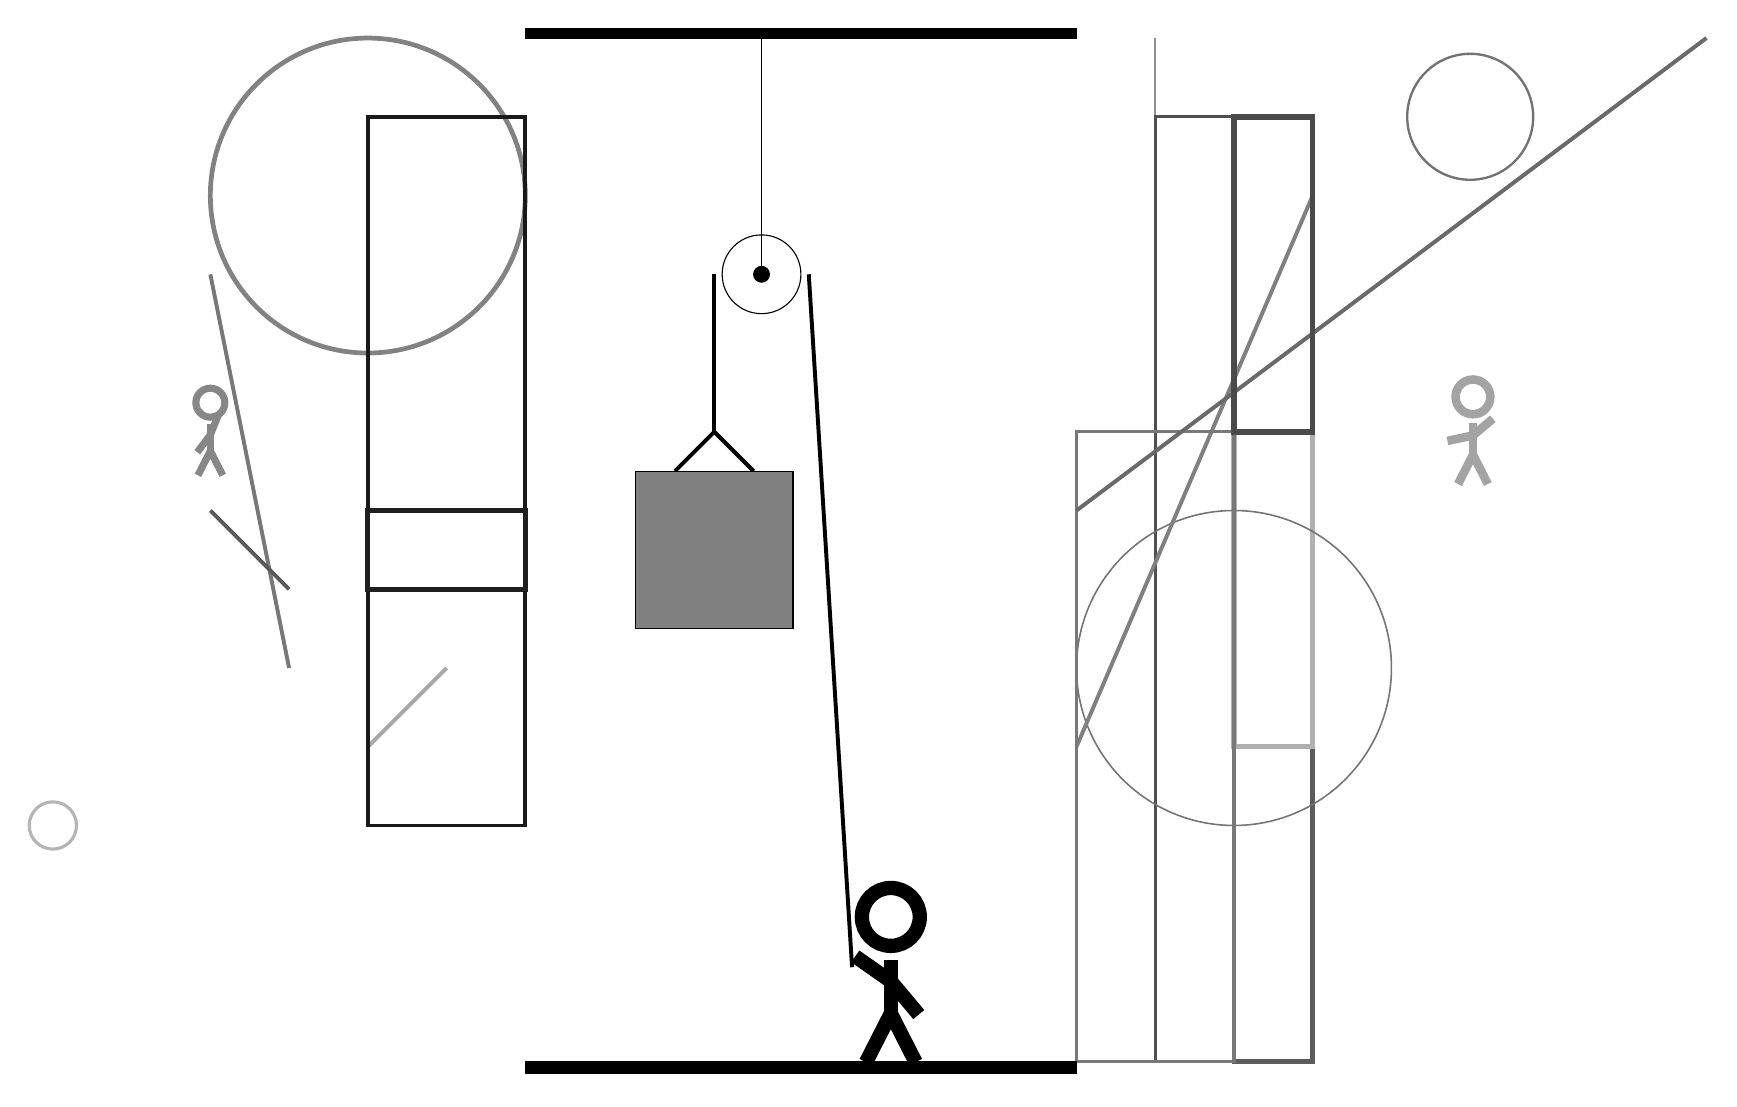
\begin{tikzpicture}
		%%%%% START %%%%%
		
		\draw[fill=black] (-2, 10) rectangle (5, 10.125);
		
		\draw (1, 7) circle (0.5);
		\draw[fill=black] (1, 7) circle (0.1);
		\draw (1, 10) -- (1, 7);
		
		\draw[line width=0.5mm] (-0.1, 4.5) -- (0.4, 5.0) -- (0.9, 4.5);
		\draw[fill=black!50] (-0.6, 4.5) rectangle (1.4, 2.5);
		
		\draw[line width=0.5mm] (0.4, 7) -- (0.4, 5.0);
		\centerarc[line width=0.5mm](1, 7)(0:180:0.6);
		\draw[line width=0.5mm](1.6, 7) -- (2.15, -1.8);
		
		\node at (2.6, -1.9) {\Strichmaxerl[10][-35][-50]};
		
		\draw [line width=0.3mm, color=black!55](10, 9) circle (0.8);
		
		\draw[line width=0.5mm, color=black!53](-5, 2) -- (-6, 7);
		\draw[line width=0.3mm, color=black!44] (6, -1) rectangle (6, 10);
		\draw[line width=0.4mm, color=black!69] (7, -3) rectangle (6, 9);
		
		\draw[line width=0.6mm, color=black!64] (7, 1) rectangle (8, -3);
		\draw[line width=0.5mm, color=black!34](-3, 2) -- (-4, 1);
		
		\draw[line width=0.5mm, color=black!65](-6, 4) -- (-5, 3);
		\draw[line width=0.7mm, color=black!31] (7, 1) rectangle (8, 9);
		\draw [line width=0.6mm, color=black!49](-4, 8) circle (2.0);
		\draw[line width=0.5mm, color=black!90] (-4, 0) rectangle (-2, 9);
		\draw[line width=0.6mm, color=black!88] (-4, 3) rectangle (-2, 4);
		\node[line width=0.6mm, color=black!36] at (10, 5) {\Strichmaxerl[6][12][40]};
		\draw [line width=0.4mm, color=black!29](-8, 0) circle (0.3);
		
		\draw [line width=0.2mm, color=black!55](7, 2) circle (2.0);
		\draw[line width=0.5mm, color=black!50](8, 8) -- (5, 1);
		\draw [line width=0.7mm, color=black!88](8, 3) circle (0.0);
		
		\draw[line width=0.4mm, color=black!53] (7, 5) rectangle (5, -3);
		\draw[line width=0.5mm, color=black!59](5, 4) -- (13, 10);
		\draw[line width=0.7mm, color=black!71] (7, 5) rectangle (8, 9);
		
		\node[line width=0.2mm, color=black!47] at (-6, 5) {\Strichmaxerl[5][53][68]};
		
		\draw[fill=black] (-2, -3) rectangle (5, -3.15);
		
		%%%%% END %%%%%
	\end{tikzpicture}
\end{document}